\documentclass[../main.tex]{subfiles}
\graphicspath{{\subfix{../IMAGES/}}}

\begin{document}
\localtableofcontents

\subsection{Technical aspects of energy}
Energy is simply a certain quantity that has been observed as remaining constant during physical, chemical and/or biological changes : \begin{equation}
    \Delta E = Q + W = \Delta U + \Delta E_p + \Delta E_k = Q + W_{sh} - W_{PV} \: \text{For a closed system \warning}
\end{equation}
with $\Delta E$ the change in energy content of the system, $Q$ the heat transferred to the system from its surroundings and $W$ the work done on the system by its surroundings. $\Delta U$ is the change in internal energy, $\Delta E_p$ the potential energy, $\Delta E_k$ the kinetic energy, $W_{sh}$ the shaft work and $W_{PV}$ the Pressure-volume work.\\

\begin{equation}
    W_{PV} = \int PdV
\end{equation}
To solve it, one uses an equation of state such as the ideal gas law : $PV = nRT$. Another one is the Van der Waals : $(P + \frac{an^2}{V^2})(V-nv) = nRT$.\\
To account for this energy, it is useful to define enthalpy (H), which includes PV : \begin{equation}\begin{gathered}
    H = U+PV\\
    \Delta U + W_{PV} = \Delta U + P\Delta V = \Delta H = Q+W_{sh} \: \text{\warning Only if constant pressure}
    \end{gathered}
\end{equation}

The absolute value for internal energy ($U_0$) is given by Einstein's expression : $U_0 = E_0 = m_0C^2$ and $\Delta U = \Delta m C^2$.\\

\quad \underline{Lower heating value :} combustion products are cooled to $150^\circ C$.\\

\quad \underline{Higher heating value :} combustion products are cooled to $25^\circ C$.\\

The major difference is water condensation : \begin{equation}
    LHV \simeq HHV - \Delta H_{vap, H2O} \frac{n_{H2O}}{n_{fuel}}
\end{equation}

\begin{table}[hbt!]
    \centering
    \begin{tabular}{c|c|c}
        Fuel & HHV [MJ/kg] & LHV [MJ/kg] \\ \hline
        $H_2$ & 142 & 120\\
        NG & 55 & 49\\
        Gasoline & 47& 43\\
        Diesel & 46 & 43\\
        Ethanol & 30 & 27\\
        Butanol & 37 & 34\\
        Wood & 21 & 20\\
        Grasses & 18 & 17\\
    \end{tabular}
\end{table}


\textbf{Entropy} is the measure of system disorder or total inventory of random information. The second law of thermodynamics states that : \begin{equation}
\begin{gathered}
    \Delta S_{system} \geq 0 \: \text{For isolated systems}\\
    \Delta S_{system} + \Delta S_{surroundings} \geq 0 \: \text{For non-isolated systems}
    \end{gathered}
\end{equation}

The change of entropy is measured as : $\Delta S_{system} = S_2-S_1 = \int \frac{dQ_{rev}}{T}$ (during a reversible process). Since the change is reversible : $\Delta S_{system,rev} + \Delta S_{surroundings,rev} = 0$.\\
For a reversible process, there is no change in entropy and therefore the system is at equilibrium. S is a \textbf{state function}.

Many processes are cyclical/steady state. For heat to work cyclical processes, entropy is an interesting state variable for characterizing the system : $dS = \frac{dQ_{rev}}{T}$ where $Q_{rev}$ is the greatest amount of heat that can be received for a given change in entropy. However, one cannot recover all of this entropy as heat : $dS > \frac{dQ_{actual}}{T}$.\\

For a cycle, $\Delta U = 0$ it is a state variable! $\Rightarrow Q = -W$. Then : $Q_{rev} = -W_{rev} = -\int T dS$.\\

\subsubsection{Carnot cycle}
Heat engine. Get heat from a hot source and outputs heat to a cold source as well as work : $W = Q_H-Q_C$. The efficiency is then : $\eta = \frac{W}{Q_H}$.\\
Step 1 : add heat to expand the gas isothermally at $T_H$ while doing work. Step 2 : expand the gas adiabatically until the gas reaches $T_C$ while doing more work. Step 3 : Remove heat to compress the gas isothermally at $T_C$ while providing work. Step 4 : compress the gas adiabatically until the gas temperature rises to $T_H$ while providing the necessary work.\\

For ideal gas : \begin{equation}
    \begin{gathered}
        U = f(T) \neq f(P,V)\\
        dU = C_v dT\\
        dH = C_p dT\\
        \Delta U = C_v \Delta T = \Delta H - \Delta (PV)\\
        C_p - C_v = R\\
        k = \frac{C_p}{C_v}\\
        dU = C_v dT = dW = -pdV \: \text{for adiabatic processes}\\
        \ln\frac{T_2}{T_1} = -\frac{R}{C_v} \ln \frac{V_2}{V_1} = -(k-1) \ln \frac{V_2}{V_1}\\
        (\frac{T_2}{T_1}) = (\frac{V_1}{V_2})^{k-1}\\
        (\frac{T_2}{T_1}) = (\frac{p_2}{p_1})^{\frac{k-1}{k}}\\
        (\frac{p_2}{p_1}) = (\frac{V_1}{V_2})^k\\
        \Delta S = n(C_p \ln(\frac{T_2}{T_1}) - R\ln(\frac{P_2}{P_1})) = n(C_v\ln(\frac{T_2}{T_1}) + R \ln(\frac{V_2}{V_1}))
    \end{gathered}
\end{equation}

For step 1 (isothermal expansion) : $Q_{AB} = -W_{AB} = RT_h \ln(\frac{V_B}{V_A}) = RT_h\ln(\frac{P_A}{P_B})$. For step 2 (adiabatic expansion) : $W_{BC} = C_v (T_c-T_h)$. For step 3 (isothermal compression) : $Q_{CD} = -W_{CD} = R T_c \ln \frac{P_C}{P_D}$. For step 4 (adiabatic compression) : $W_{DA} = C_v(T_h-T_c)$.\\
Then : $\eta = \frac{-W_{tot}}{Q_h}=\frac{RT_h \ln \frac{P_A}{P_B} + RT_c \ln \frac{P_C}{P_D}}{RT_H \ln \frac{P_A}{P_B}} = \frac{T_h-T_c}{T_h}$.\\

For heat pumps, use it in reverse! If used for heating $\eta_w = \frac{-Q_h}{W_{tot}} = \frac{T_h}{T_h-T_c}$, if used for cooling : $\eta_s = \frac{T_c}{T_h-T_c}$.\\

\begin{figure}[hbt!]
    \centering
    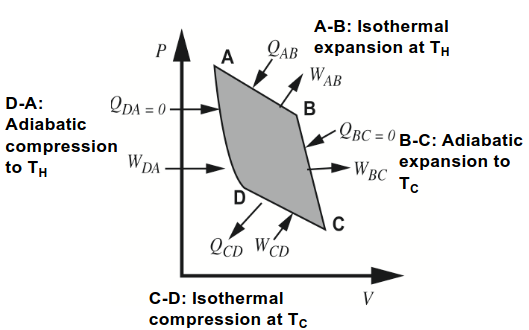
\includegraphics[width=0.5\linewidth]{IMAGES/Renewable/Screenshot from 2025-02-25 15-51-57.png}
\end{figure}
\begin{figure}[hbt!]
    \centering
    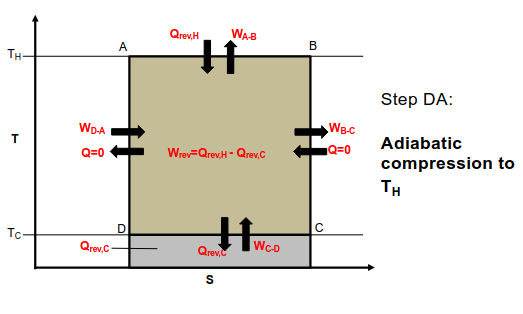
\includegraphics[width=0.5\linewidth]{IMAGES/Renewable/Screenshot from 2025-02-25 15-52-04.png}
\end{figure}

\subsubsection{Rankine cycle}

\begin{figure}[hbt!]
    \centering
    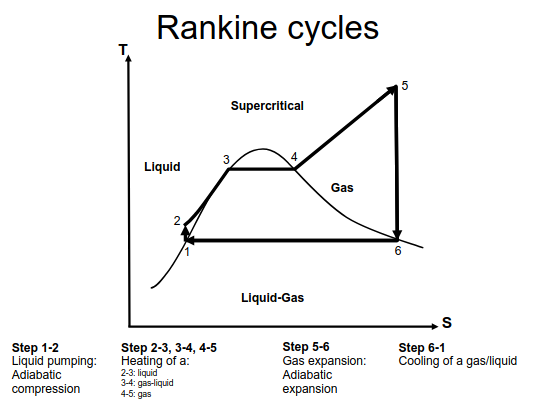
\includegraphics[width=0.5\linewidth]{IMAGES/Renewable/Screenshot from 2025-02-25 16-30-37.png}
\end{figure}

The efficiency is then : $\eta = \frac{W}{Q_h} = \frac{(H_5-H_2)-(H_6-H_1)}{H_5-H_2}$. But as the energy for compressing a liquid is small : $\eta = \frac{H_5-H_6}{H_5-H_1}$.\\
For safety, increase $T_5$ (and therefore $S_5$) in order that when the temperature decreases, it does not directly go to $T_6$ (eliminate the risk of cavitation).\\
Pumping a liquid close to a gaseous state leads to cavitation, expanding a gas-to-liquid mixture leads to erosion.\\
\warning Rankine efficiency is lower than Carnot (which is not feasible in practice), as the area is smaller. To increase efficiency : reheat steam before condensing. \\

Refrigeration cycle is basically the same in reverse. \\

\begin{figure}[hbt!]
    \centering
    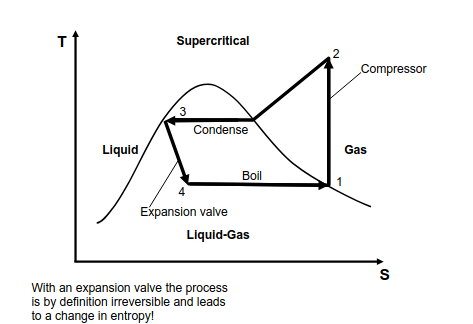
\includegraphics[width=0.5\linewidth]{IMAGES/Renewable/Screenshot from 2025-02-25 16-53-25.png}
\end{figure}

$COP_{refrigeration} = \frac{Q_c}{W} = \frac{H_1-H_4}{H_2-H_1}$ and $COP_{heat\: pump} = \frac{-Q_h}{W} = \frac{H_2-H_3}{H_2-H_1}$.\\

\subsubsection{Gasoline engines (Otto cycle)}
\begin{figure}[hbt!]
    \centering
    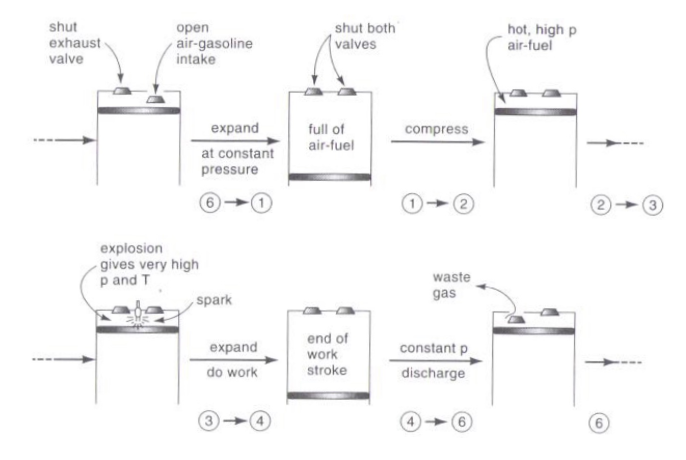
\includegraphics[width=0.5\linewidth]{IMAGES/Renewable/Screenshot from 2025-03-04 15-18-26.png}
    \caption{Otto cycle}
\end{figure}

\begin{figure}[hbt!]
\begin{minipage}{.5\textwidth}
    \centering
    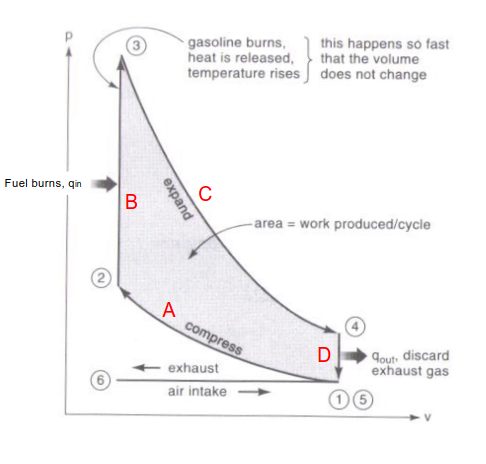
\includegraphics[width=\linewidth]{IMAGES/Renewable/Screenshot from 2025-03-04 15-21-36.png}
    \caption{pV diagram of the Otto cycle}
\end{minipage}
\hfill
\begin{minipage}{.5\textwidth}
    \centering
    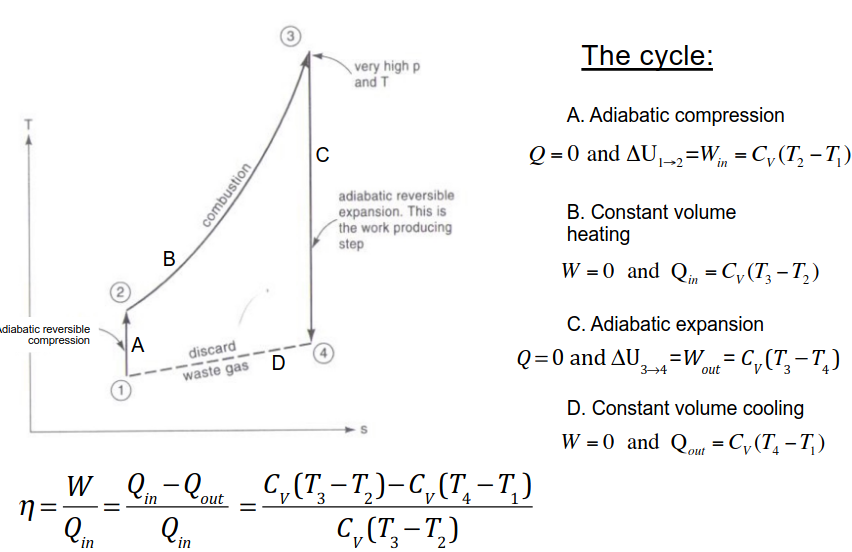
\includegraphics[width=\linewidth]{IMAGES/Renewable/Screenshot from 2025-03-04 15-22-18.png}
    \caption{TS diagram of the Otto cycle}
\end{minipage}
\end{figure}


With : $\eta = 1-\frac{T_1}{T_2} = 1- (\frac{V_2}{V_1})^{1-k} = 1-r_c^{1-k}$, $r_c = \frac{V_1}{V_2} = \frac{V_4}{V_3}$ the compression ratio. In gasoline engine : $r_c \simeq 8-9$ and $\eta=35-45\%$.\\

\subsubsection{Diesel engine}

\begin{figure}[hbt!]
\begin{minipage}{.5\textwidth}
    \centering
    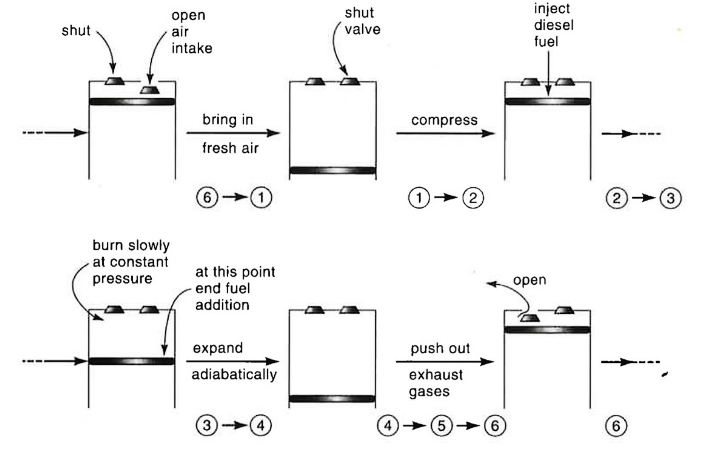
\includegraphics[width=\linewidth]{IMAGES/Renewable/Screenshot from 2025-03-04 15-35-05.png}
    \caption{Diesel cycle}
\end{minipage}
\hfill
\begin{minipage}{.5\textwidth}
    \centering
    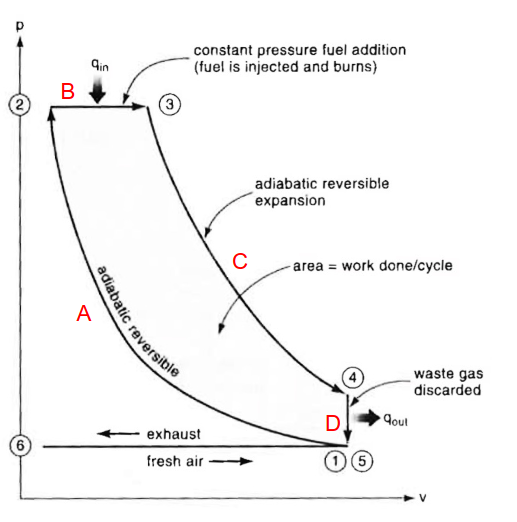
\includegraphics[width=\linewidth]{IMAGES/Renewable/Screenshot from 2025-03-04 15-38-48.png}
    \caption{pV diagram of the diesel cycle}
\end{minipage}    
\end{figure}


\begin{figure}[hbt!]
    \centering
    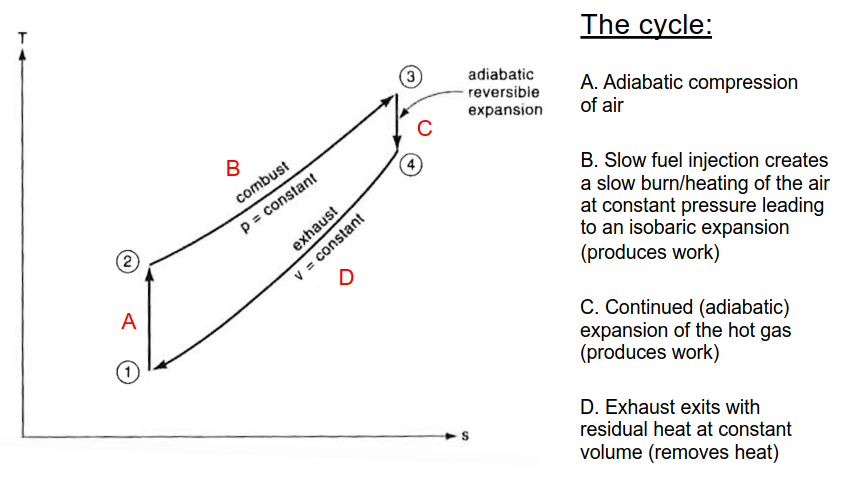
\includegraphics[width=0.5\linewidth]{IMAGES/Renewable/Screenshot from 2025-03-04 15-42-47.png}
    \caption{TS diagram of the diesel cycle}
\end{figure}

Then : $\eta = 1-\frac{1}{k} \frac{T_4-T_1}{T_3-T_2}$, with $r_c = \frac{V_1}{V_2}$ the compression ratio and $r_e = \frac{V_4}{V_3}$ the expansion ratio. This gives : $\mathbf{\eta = 1-\frac{1}{k} \frac{(\frac{1}{r_e})^k-(\frac{1}{r_c})^k}{\frac{1}{r_e}-\frac{1}{r_c}}}$.\\
For the same compression ratio, Otto cycle is more efficient but in practice, diesel engine have a higher compression ratio ($r_c\simeq 20$).\\

\subsubsection{Brayton cycle}
Used for gas turbines and jet engines. \\

\begin{figure}[hbt!]
\begin{minipage}{.5\textwidth}
    \centering
    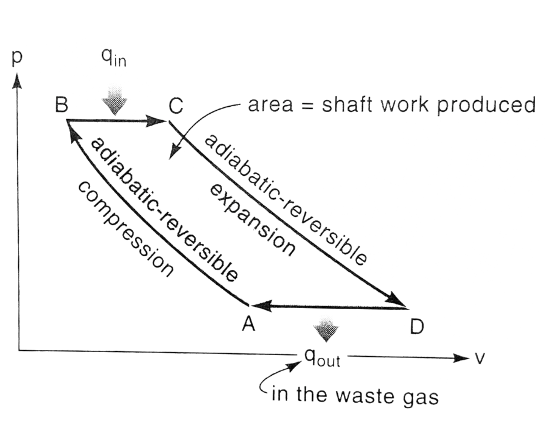
\includegraphics[width=\linewidth]{IMAGES/Renewable/Screenshot from 2025-03-04 17-16-30.png}
    \caption{Brayton cycle pV diagram}
\end{minipage}
\hfill
\begin{minipage}{.5\textwidth}
    \centering
    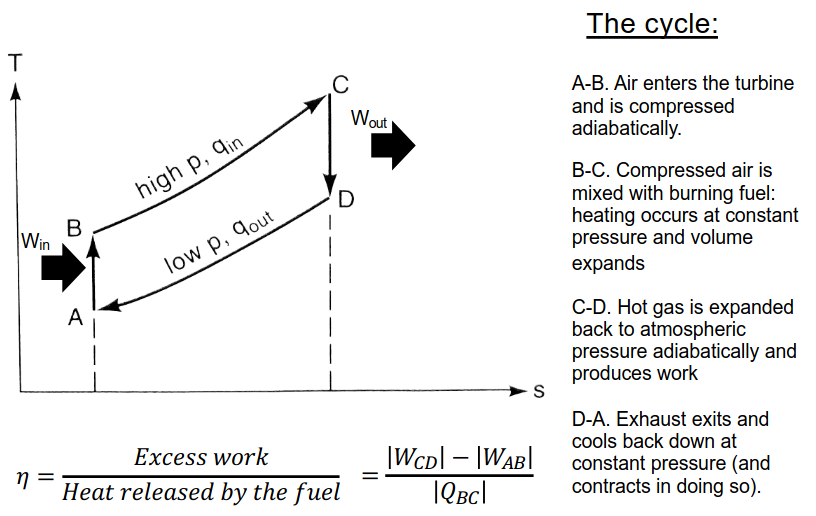
\includegraphics[width=\linewidth]{IMAGES/Renewable/Screenshot from 2025-03-04 17-17-56.png}
    \caption{Brayton cycle TS diagram}
\end{minipage}
\end{figure}

The efficiency is then : $\eta = 1-\frac{T_A}{T_B} = 1-(\frac{P_A}{P_B})^{\frac{k-1}{k}}$. Pressure ratios are around 20 and theoretical efficiencies are around 55-60\%.\\

For jet engines : same idea such that it accelerates the exiting gas. Its efficiency is : $\eta = \frac{\text{propulsive power}}{\dot{Q}_{in}} = \eta_{th} \eta_{propulsive}$. With : $\eta_{th} = 1-\frac{T_A}{T_B}$ the ratio of kinetic energy created over the thermal energy given by the fuel, and $\eta_{propulsive} = \frac{\text{propulsive power}}{\text{rate of production of propulsive kinetic energy}} = \frac{v_{in} \dot{m}_{air} (v_{out}-v_{in})}{\dot{m}_{air} (v_{out}^2-v_{in}^2)/2} = \frac{2}{1+ \frac{v_{out}}{v_{in}}}$ the ratio of propulsive power produced by the rate of production of kinetic energy transferred into the gas.\\
By increasing the air flow, the efficiency does not change but thrust increases, while increasing the difference in air velocity (out-in) increases thrust but decreases efficiency.\\

\subsubsection{Exergy}
Exergy is the maximum amount of useful work obtainable for a given process. $dW_{ex} = dW_{sh} + dW_0 = -dE + T_0dS -p_0dV \Rightarrow W_{Ex} = \Delta U + E_p + E_k + T_0 \Delta S - p_0(V_0-V_1) = \Delta H + E_p + E_k + T_0 \Delta S$.\\

\warning The free gibbs energy is : $G = U-TS+PV$, for a fuel that starts out at $T_0$, $P_0$ then $W_{ex} = -\Delta G_0$. Only for a fuel.\\

Then : \begin{equation}
    W_{ex, 1-2} = W_{ex,1-0} - W_{ex,2-0} = -(E_2-E_1) + T_0(S_2-S_1) - p_0(V_2-V_1)
\end{equation}

\begin{figure}[hbt!]
    \centering
    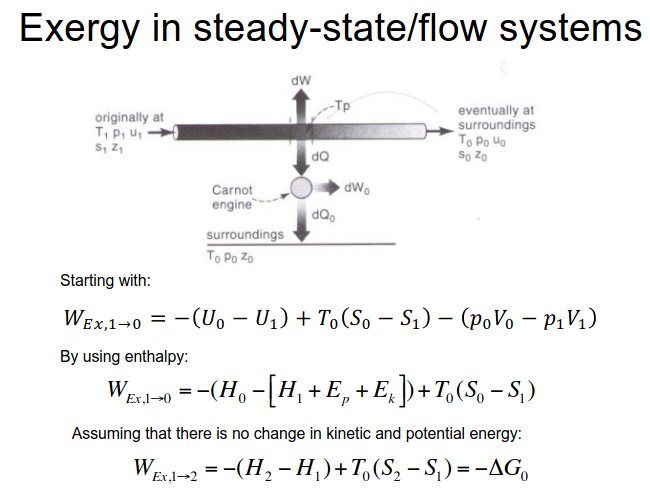
\includegraphics[width=0.8\linewidth]{IMAGES/ESE/Screenshot from 2025-03-11 15-38-32.png}
\end{figure}

The work lost in a real process is then : $W_{sh,lost} = T_0 \Delta S_{tot}$.\\

\subsubsection{Fuel cells}
The fuel oxidation involves the exchange of electrons : $H_2 + \frac{1}{2} O_2 \rightleftharpoons H_2 O$. This reaction can be separated into two half reactions : $H_2 \rightleftharpoons  2H^++2e^-$ and $\frac{1}{2}O_2 +2H^+ +2e^- \rightleftharpoons H_2O$.\\

\begin{figure}[hbt!]
    \centering
    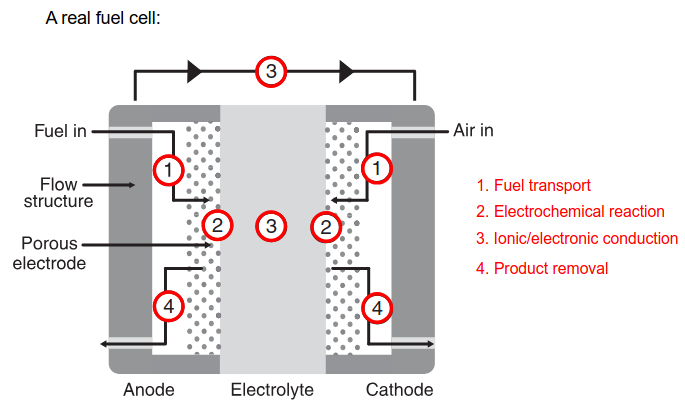
\includegraphics[width=0.5\linewidth]{IMAGES/ESE/Screenshot from 2025-03-11 16-21-36.png}
\end{figure}

In general, extensive properties are more difficult to change than intensive properties. \\
To describe another thermodynamic potential : use \textbf{Legendre transformation}. Start with $dU = TdS - PdV  + \mu dN$. Then : $d(U+PV) = dH = TdS + VdP + \mu dN$ (with H the enthalpy). Also : $d(U+PV-TS) = dG = -SdT + VdP +\mu dN$ (with G the free gibbs energy) and $d(U-TS) = dF = -SdT -PdV+ \mu dN$ (with F the Hemholtz energy).\\
\warning PV can be interpreted physically as the work needed to create volume for the system to exist. TS can be interpreted as the energy required to be exchanged with the environment.\\

\begin{figure}[hbt!]
    \centering
    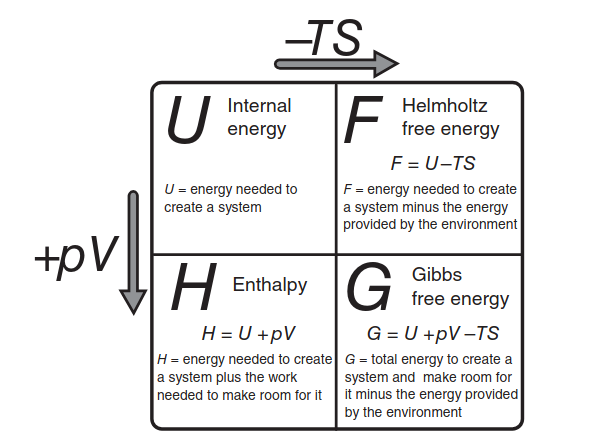
\includegraphics[width=0.6\linewidth]{IMAGES/ESE/Screenshot from 2025-03-11 16-36-43.png}
\end{figure}

For fuel cells : $dU = dQ - dW_{electric} - dW_{PV}$, in the best case : $dQ  =TdS$. From free energy : $dG = dU-SdT-TdS+PdV+VdP = -SdT + VdP -dW_{elec}$. At constant P and T : $dG = -dW_{elec}$. Therefore, for a given oxidation : $W_{elec} = -\Delta G_{RXN}$.\\
The efficiency is then \begin{equation}
    \eta = \frac{W_{elec}}{\text{Total energy}} = \frac{\Delta G_{RXN}}{\Delta H_{RXN}} = 1-\frac{T\Delta S_{RXN}}{\Delta H_{RXN}}
\end{equation}

For hydrogen ($\Delta H = -286kJ/mol$, $\Delta G = -237 kJ/mol$) then : $\eta = 83\%$.\\

For the rare cases where entropy is positive the efficiency is above $100\%$. In this case : $\eta = \frac{W_{elec}}{\text{Energy from RX + heat received}} = 1$. \\

\quad \underline{Reversible voltage :}\\
The electrical work of moving charge q is : $W_{elec} = qE$. We have : $q=nF$. Also : $W_{elec} = -\Delta G_{RXN}$. Then : $E^0 = -\frac{\Delta G_{RXN}}{nF}$ (for Fuel cell : $E_0 = 1.23V$).\\

\subsection{Systems modeling}
Processes are assemblies of interconnected unit operations. Process models are usually represented as Flowsheets. \\
Types of stream : Heat stream (characterized by their energetic flux, for heat integration the temperature of heat exchange is needed), Non-heat energetic stream (mechanical and electrical, characterized by their energetic power), Material stream (characterized by either intensive/extensive properties, it is completely characterized if $N_{sp} = N_{spi} + N_{spe} = 2+N_c$ or number of required species properties = number of specified intensive + extensive properties = 2+number of components in the stream and $N_{spe} \geq 1$).\\
How many intensive variables can be specified independently of each other : (Gibbs phase rule) $F_{int} = 2+N_c-N_p$, or degree of freedom for intensive variable = 2+ number of components in the stream - number of phases.\\

Stream properties : total number of specification $N_{specification} = N_{streams, Q} + N_{streams, W_{El}} + 2 N_{streams, W_{mech}} + N_{streams, material} (2+N_c)$ or total number of specification = heat streams + electrical streams + mechanical work streams (2 per stream) + material streams.\\
An overall specification matrix S is constructed by putting together all of these stream matrices.\\
\warning This number of specifications is only needed for isolated streams. Units connected these streams will reduce their degree of freedom.\\

\subsubsection{Pure component properties in ideal conditions}
\begin{equation}
\log(P_{sat,\alpha}) = A_\alpha - (\frac{B_\alpha}{T_{sat,\alpha} + C_\alpha})
\end{equation}
Antoine's equation.\\

Enthalpy :\\
\quad \underline{Gas phase :} $\Delta H = \Delta H_f + \Delta H_p + \Delta H_T$, with $\Delta H_f$ the enthalpy of formation (findable in a database), assume $\Delta H_p = 0$ and $\Delta H_T(T) = \int_{T_0}^T C_p(T')dT'$ with $C_p(T') = A_\alpha + B_\alpha T + C_\alpha T^2 + D_\alpha T^3 + \frac{E_\alpha}{T^2}$.\\

\quad \underline{Liquid phase :} $\Delta H = \Delta H_f + \Delta H_T - \Delta H_{vap}$, with $\Delta H_{vap}(T) = \Delta H_{vap} (T_{\alpha,b}) (\frac{T_{\alpha,c} - T}{T_{\alpha,c}-T_{\alpha,b}})^{\eta\simeq 0.38} $.\\

Entropy :\\
\quad \underline{Gas phase :} entropy does not need a reference state. It has an absolute value based on a perfect crystal at $0K$ : $\Delta S_{v,\alpha} (T,P) = S_{0,\alpha} + \int_{T_0}^T \frac{C_{p\alpha} (T')}{T'} dT' - R\ln \frac{P}{P_0}$.\\

\quad \underline{Liquid phase :} $\Delta S_{v,\alpha} (T,P) = S_{0,\alpha} + \int_{T_0}^T \frac{C_{p\alpha} (T')}{T'} dT' - R\ln \frac{P}{P_0} - \Delta S_{vap,\alpha} (T)$, with $\Delta S_{vap,\alpha} (T) = \frac{\Delta H_{vap,\alpha}(T)}{T}$.\\

\subsubsection{Ideal mixtures}
In ideal mixtures, U and H are additive : $U = \sum U_\alpha$ (same for H).\\
For entropy we have to take into account the entropy of mixing : $S = \sum x_\alpha S_\alpha - \sum x_\alpha R \ln x_\alpha$.\\
The Gibbs free energy is then simply : $G = H-TS$.\\

\quad \underline{Vapor liquid equilibrium :}\\
We want to find the state at equilibrium : $dG=0 \Rightarrow dG = -SdT + VdP + \sum_p \sum_\alpha \mu_{p,\alpha} dn_{p,\alpha}$, with p the phases and $\alpha$ the component.\\

If T and P are constant : \begin{equation}
    \begin{gathered}
        dG = -SdT+ VdP + \sum_p \sum_\alpha \mu_{p,\alpha} dn_{p,\alpha} = \sum_p \sum_\alpha \mu_{p,\alpha} dn_{p,\alpha} = 0\\
        (\frac{dG}{dn_\alpha}) = 0 \Rightarrow \sum_p \mu_{p,\alpha} = 0\\
        \Rightarrow \mu_{1,\alpha} = \mu_{2,\alpha} = \cdots\\
    \end{gathered}
\end{equation}

\warning the chemical potentials of each component must be equal across all phases.\\
For a vapor-liquid equilibrium : $\mu_{V,\alpha} = \mu_{L,\alpha} = \mu_{L,\alpha}^0 + RT \ln \frac{f_{\alpha,L}}{f_{\alpha,L}^0}$. The reference state for $\mu_\alpha^0$ and $f_\alpha^0$ is arbitrary. Let $f_{V,\alpha}$ be the fugacity. From equilibrium, $f_{V,\alpha} = f_{L,\alpha}$.\\
They can be defined as : $f_{V,\alpha} = \varphi_{\alpha,V} y_\alpha P$ and $f_{L,\alpha} = \varphi_{\alpha,L} x_\alpha P = \gamma_\alpha x_\alpha f_{L,\alpha}^0$ ($x_\alpha$ and $y_\alpha$ the molar fraction). Then : $f_{L,\alpha}^0 = \varphi_{\alpha,L}P$, with $\varphi_\alpha = \exp(\int_0^P \frac{\nu_\alpha}{RT}-\frac{1}{P}dP)$. Finally, $\varphi_{\alpha,V}y_\alpha P = \gamma_\alpha x_\alpha \varphi_{\alpha,L}^{sat} P_{sat} \exp(\int_{P_{sat}}^P \frac{\nu_{L,\alpha}}{RT}dP)$. Simplifications : ideal solution ($\gamma=1$), ideal gas ($\varphi=1$), incompressible liquids (exp to 1). Then : $y_\alpha P = x_\alpha P_{sat}$ (Raoult's law).\\

\warning Some approximations are not always true : $\gamma$ isn't always 1.\\

\quad \underline{Strategy 1 : activity coefficient models}\\
$\overline{G} = \overline{G}_{Id} + \overline{G}_E$, with $\overline{G}_E$ the excess partial molar Gibbs free energy, with $\overline{G}_\alpha= (\frac{\partial G}{\partial n_\alpha})_{T,P,n_{\alpha \neq \beta}}$. Then : $\overline{G}_{E,\alpha} = RT \ln \gamma_\alpha = \frac{\partial}{\partial n_\alpha} [(\sum n_k)(\overline{G}_E)] =  \frac{\partial}{\partial n_\alpha} [(\sum n_k)(f(x_\alpha,x_\beta, \cdots, T))]$.\\
$\overline{V}_{E,L}=(\frac{\partial \overline{G}_{E,L}}{\partial P})_T$, $\Delta \overline{S}_{E,L}=-(\frac{\partial \overline{G}_{E,L}}{\partial T})_P$ and $\Delta \overline{H}_{E,L} = \Delta \overline{G}_{E,L} +T\Delta \overline{S}_{E,L}$.\\

\quad \underline{Strategy 2 : Equation of State models}\\
We start with volumetric properties and arrive at thermodynamic properties. \\
\begin{figure}[hbt!]
    \centering
    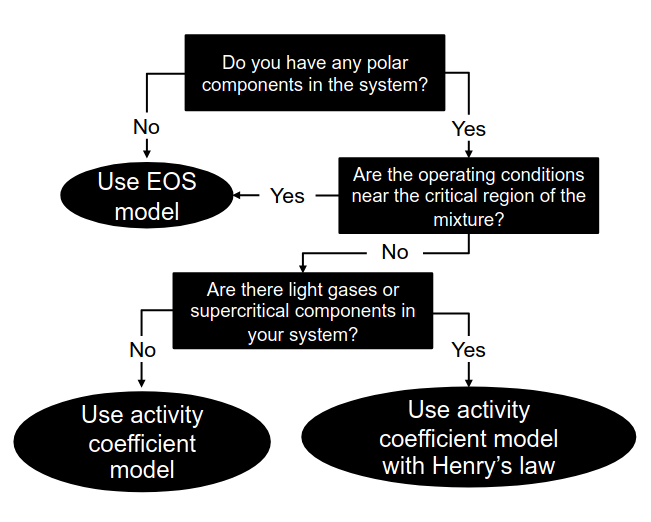
\includegraphics[width=0.5\linewidth]{IMAGES/ESE/Screenshot from 2025-03-25 16-00-17.png}
    \caption{Choosing your thermodynamic property estimation method}
\end{figure}

We can use all of the relations to construct the matrix $Th_a$ (for stream a) such that $Th_a(T_a, P_a, Cp_a, h_a, z_{\alpha,a},\cdots)=0$.

\subsubsection{Unit models}
Provides connectivity and unit-specific relationships.\\

Basic balance structure : In-Out = Accumulation + Source.\\
Balances form their own matrix $U_i$ such that $U_i (T_a,P_a, h_a, \cdots, P_{i1},\cdots)=0$. An overall specification matrix U is constructed by putting together all of these unit matrices. We can now build an overall set of equations using stream properties, thermodynamics relationships and unit models : $F = \begin{pmatrix}
    S_a\\ S_b \\ \vdots\\ Th_a\\Th_b\\ \vdots \\ U_i \\ U_j \\ \vdots \\
\end{pmatrix} = 0$. \warning The matrix must be squared, equations must be independent.\\

\subsubsection{Energy integration}
Energy integration is the concept of recovering and valorizing heat within a process.\\
Pinch analysis is a systematic method for performing heat integration. It calculates the minimum heating/cooling requirements. Use of a heat exchanger for example. Limitations : temperature difference is the driving force and 1st law of thermodynamics (heat loads are conserved).\\
Heat load calculation : $Q = \Delta H = C_p (T_2-T_1)$. One can then derive : $T_2 = T_1 + \frac{1}{C_p}(\Delta H_0 + \Delta H)$.

\begin{figure}[hbt!]
    \centering
    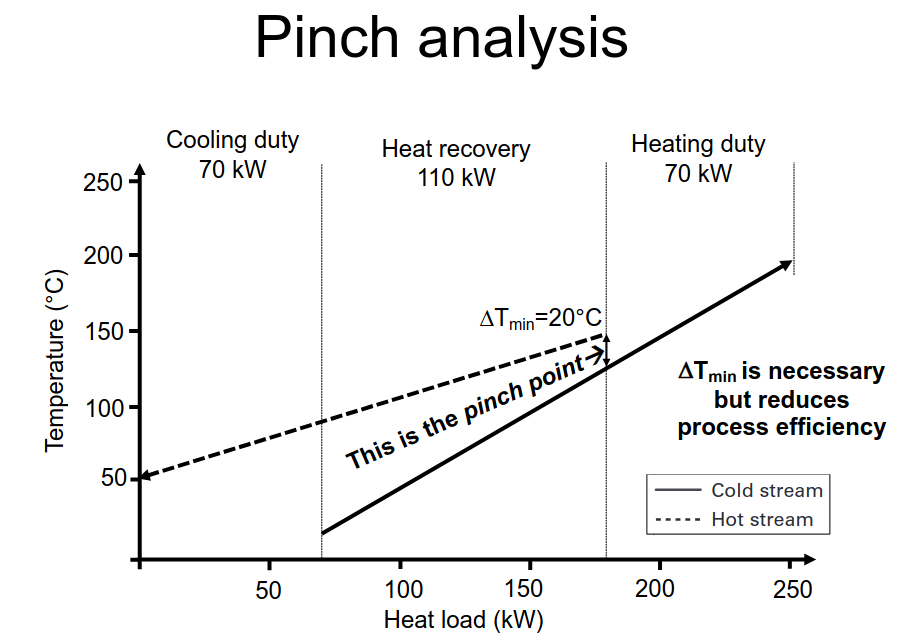
\includegraphics[width=0.5\linewidth]{IMAGES/ESE/Screenshot from 2025-03-25 18-00-40.png}
\end{figure}

Rule of thumbs for $\Delta T_{min}$ : $8^\circ C$ for gases, $4^\circ C$ for liquids, $2^\circ C$ for evaporating/condensing streams and $25^\circ C$ for reacting streams. For multi-stream process : compute the Q for each T interval. \\

How to apply the graphical method with a computer? \\
Heat cascade using Thermal stream matrix : $Ts = \begin{pmatrix}
        T_{i,in} & T_{i,out} & Q_i\\ T_{j,in} & T_{j,out} & Q_j \\ \cdots & \cdots & \cdots\\
    \end{pmatrix}$. For continuous processes it is computed with $Q_i = H_{i,out} - H_{i,in}$. If $Q_i>0$ heat is received (cold stream), otherwise heat is removed (hot stream). For cold streams : $T_i^* = T_i + \frac{\Delta T_{min}}{2}$ and for hot stream : $T_i^* = T_i - \frac{\Delta T_{min}}{2}$ and put them in the $Ts'$ matrix. This makes it easier to identify the pinch. $C_p$ is then computed as : $C_{pi} = \frac{\lvert Q_i \rvert}{\lvert T_{i,in}-T_{i,out} \rvert}$. This allows to linearize $C_p$ for each heat exchange.\\
Then : $Ts' = \begin{pmatrix}
    T_{i,in}^{'*} & T_{i,out}^{'*} & C_{pi}\\ 
    T_{j,in}^{'*} & T_{j,out}^{'*} & C_{ji}\\ 
    \cdots & \cdots & \cdots\\
\end{pmatrix}$
    \warning For a phase change $\Delta T =0$ so $C_p=\infty$; two options : identify and treat phase change separately, easier algorithm ($T_{i,out}^* = T_{i,out}^* + \Delta T_{min}/1000$).\\
We start with the highest $T$ and cascade down. Then we identify all the units that operates for a given T interval. To do that, we identify the relevant lines in $Ts'$ for interval k which we call $T_{rel,k}$ such that : $T_{rel,k} = Ts'$ for which $Ts'(i,high)>T_{int}(k,2)$ and $Ts'(i,low)< T_{int} (k,1)$. With $T_{int}$ the 2xn matrix that contains all the unique temperatures. With this, we sum up the relevant $C_p$ (for cold stream : $C_p<0$) to compute the heat in interval k : $Q_k = \sum \pm C_p (T_{high}-T_{low}) = \sum_i [T_{rel,k}(i,3) (-\frac{Q_i}{\lvert Q_i \rvert })] (T_{int}(1,k)-T_{int}(2,k)]$. The cascade heat is then : $Q_{c,k} = \sum Q_k$.\\
$T_{int} = \begin{pmatrix}
    T_1^* & T_2^*\\ T_2^* & T_3^*\\ \cdots & \cdots \\
\end{pmatrix}$ ordered in decreasing order.\\


\warning The lowest value of $Q_{c,k}$ is the pinch point. As we want the cascaded heat to be positive and zero at the pinch : $Q_{c,k}' = Q_{c,k} + \lvert min(Q_{c,k}) \rvert$.\\
This is called the Grand Composite Curve : $GCC = \begin{pmatrix}
    T_{int}(1,1) & \lvert min(Q_{c,k}) \rvert\\ T_{int}(1,2) & Q_{c,1}'\\ T_{int}(2,2) & Q_{c,2}'\\ \cdots &\cdots\\ T_{int}(n,2) & Q_{c,n}'\\
\end{pmatrix}$. We have to fit all hot utilities above the curve and all cold utilities below the curve. \\

Using the two composite curves we can compute a minimum heat exchanger area : (break up the curve into segments of constant $C_p$) $A_{min} = \sum A_i = \sum_i \frac{Q_i}{U_i \Delta T_{lm,i}}$ with the logarithmic mean temperature : $\Delta T_{lm,i} = \frac{(T_{h,in} -T_{c,out} + \Delta T_{min}) - (T_{h,out} - T_{c,in} + \Delta T_{min})}{\ln(\frac{T_{h,in}-T_{c,out} + \Delta T_{min}}{T_{h,out} - T_{c,in} + \Delta T_{min}})}$.\\

\subsection{LCA}
\textbf{Cradle-to-grave :} used for comparing different products. \textbf{Cradle-to-gate :} used for comparing different processes. \\
LCA is performed in 3 phases : goal and scope definition (before modeling), LCI (builk of the modeling), LCIA (links modeling input-output with environmental impact models).\\

\begin{itemize}
    \item Goal and scope : Functional unit defines scope and boundaries (geographical, use, assumptions, ...)
    \item LCI : find all activites ,intermediate exchanges, elementary exchanges (direct exchange with the environment, can be broken down into 3 categories : land use, resource consumed and emissions)
    \item LCIA : translates the elemental exchanges into 1 or several environmental impacts. Basic procedure : classification (elementary exchange are grouped into impact categories), characterization (calculation of the category impact from the exchanges classified in this category), normalization/grouping/weighting (category impacts are aggregated together into a single or several environmental impact indicators).
\end{itemize}

\subsection{Uncertainty analysis}
Uncertainty can shape the conclusions. You can measure the uncertainty of the inputs/parameters. Analytically : $\sigma_e^2 = \sum_i (\frac{\delta e}{\delta x_i}) \sigma_{x_i}^2$, $\sigma_e$ the cumulative variance of e, $\delta e$ dependent variable of interest e, $\delta x_i$ independent variable $x_i$, $\sigma_{x_i}$ the variance of $x_i$. However, for a complex system there is no analytical function : The Monte Carlo.\\
The \textbf{Monte Carlo} method is brute force method for calculating the unknown probability distribution of a dependent variable e from a set of known probability distributions of variables z. \\
4 steps : \begin{enumerate}
    \item Build a probability distribution function and cumulative probability distribution for each independent variable
    \item The cumulative distribution function is used to generate a random value of each variable z that follows it's probability distribution
    \item Do this for all independent variables and calculate the dependent variable using your model
    \item Construct a probability distribution based on a histogram of your output data. $\overline{e} = \frac{\sum_j e_j}{N}$, $\sigma_e^2 = \frac{\sum_j (e_j-\overline{e})^2}{N(N-1)}$.\\
\end{enumerate}

\subsection{Economics}
\quad \underline{Capital cost :}\\
Accounting for capacity : $C_Q = C_B (\frac{Q}{Q_B})^M$, $C_Q$ the equipment cost at capacity Q, $C_B$ the equipment cost at base capacity, M the equipment-dependent exponent, $Q_B$ the base capacity. \\
Correcting for the age of the data : (equipment costs evolve due to change inflation) $C_i = C_j (\frac{Index_i}{Index_j})$.\\
Correction factors : $C_{Q,corr} = C_B (\frac{Q}{Q_B})^M f_M f_Tf_P$, $f_M$ the mx correction factor, $f_P$ the design pressure correction, $f_T$ the design temperature correction. \\
Typical costs : raw mx (RM, chemicals, catalysts, ...), utilities costs (U, fuel, electricity, steam, ...), taxes (T). $T = (P-D)t_R$, $P$ the gross profit, $D$ the deductions and $t_R$ the tax rate. Operating labor cost (L), supervision (0.25L), overhead (0.5(L+supervision)), maintenance (0.02 $C_{total}$), rent of land ($0.02C_{total}$), plant overhead ($0.65 (L+supervision+overhead)+maintenance$).\\

Externalities are an indirect cost or benefit to an uninvolved third party. They are often used to refer to the cost of environmental damages caused by the technology. Two way of dealing with them : pay for the damages (SF), impose an upfront tax to encourage abatement ($GHG_{tax}$). \\
Total costs are : Total cost = $\sum_i RM_i + \sum_j U_j + T + L + supervision+ overhead+maintenance+rent+plant\: overhead+SF+GHG_{tax}$.\\

\quad \underline{Time and money :}\\
The value of money changes depending on when it is available because any money spent now cannot be used to earn interest in a bank/investment. Let F be the future worth, P the present cash flow and i the interest : $F = Pe^{i_ct}$. This is for continuous interest. For interest computed n times per year : $F = P(1+\frac{i_d}{n})^t$.\\
The continuous and discrete compounding are linked by : $i_c = \ln(1+\frac{i_d}{n})^n$.\\
The levelized annual rate of expenditures A for a given continuous interest $i_c$ is then : $P_T = \int_0^T A e^{-i_ct}dt$, or : $A = \frac{i_c}{1-e^{i_cT}} P_T$.\\
Procedure to compute the rate of return of a process to make a given return : determine the cash flow, bring all cash flows back to time zero and sum them up ($P_T = \sum_j F_j e^{-i_cj} = \sum_j \frac{F_j}{(1+i_d/n)^j}$), choose $i_c/i_d$ or alternatively the minimum selling price such that $P_T = 0$, if of interest redistribute all cash flows over the appropriate time horizon to calculate the levelized costs and revenue ($A = \frac{i_c \sum_j F_j}{1-e^{i_cT}}$).

\end{document}